\documentclass{beamer}
\usepackage[dutch]{babel}
\usepackage{calc}
\usepackage[absolute,overlay]{textpos}
\usepackage{amsmath}
\usepackage{amsthm}
\usepackage{graphicx}
\usepackage{tikz}
\usetikzlibrary{decorations.pathreplacing}
\mode<presentation>{\usetheme{tud}}

\title[NedTrain Planner]{NedTrain Planner}
%\subtitle
\institute[TU Delft]{Technische Universiteit Delft}
\author{Chris Bakker, Anton Bouter, Martijn den Hoedt}
\date{2 juli 2014}

\theoremstyle{definition}
\newtheorem{definitie}{Definitie}[section]

% Insert frame before each subsection (requires 2 latex runs)
\AtBeginSubsection[] {
	\begin{frame}<beamer>\frametitle{\titleSubsec}
		\tableofcontents[currentsection,currentsubsection]  % Generation of the Table of Contents
	\end{frame}
}
% Define the title of each inserted pre-subsection frame
\newcommand*\titleSubsec{Next Subsection}
% Define the title of the "Table of Contents" frame
\newcommand*\titleTOC{Outline}

% define a symbol which can be removed if you don't need it
\newcommand{\field}[1]{\mathbb{#1}}
\newcommand{\Zset}{\field{Z}}

\tikzset{
  invisible/.style={opacity=0},
  visible on/.style={alt={#1{}{invisible}}},
  alt/.code args={<#1>#2#3}{%
    \alt<#1>{\pgfkeysalso{#2}}{\pgfkeysalso{#3}} % \pgfkeysalso doesn't change the path
  },
}

\begin{document}

{
% remove the next line if you don't want a background image
\usebackgroundtemplate{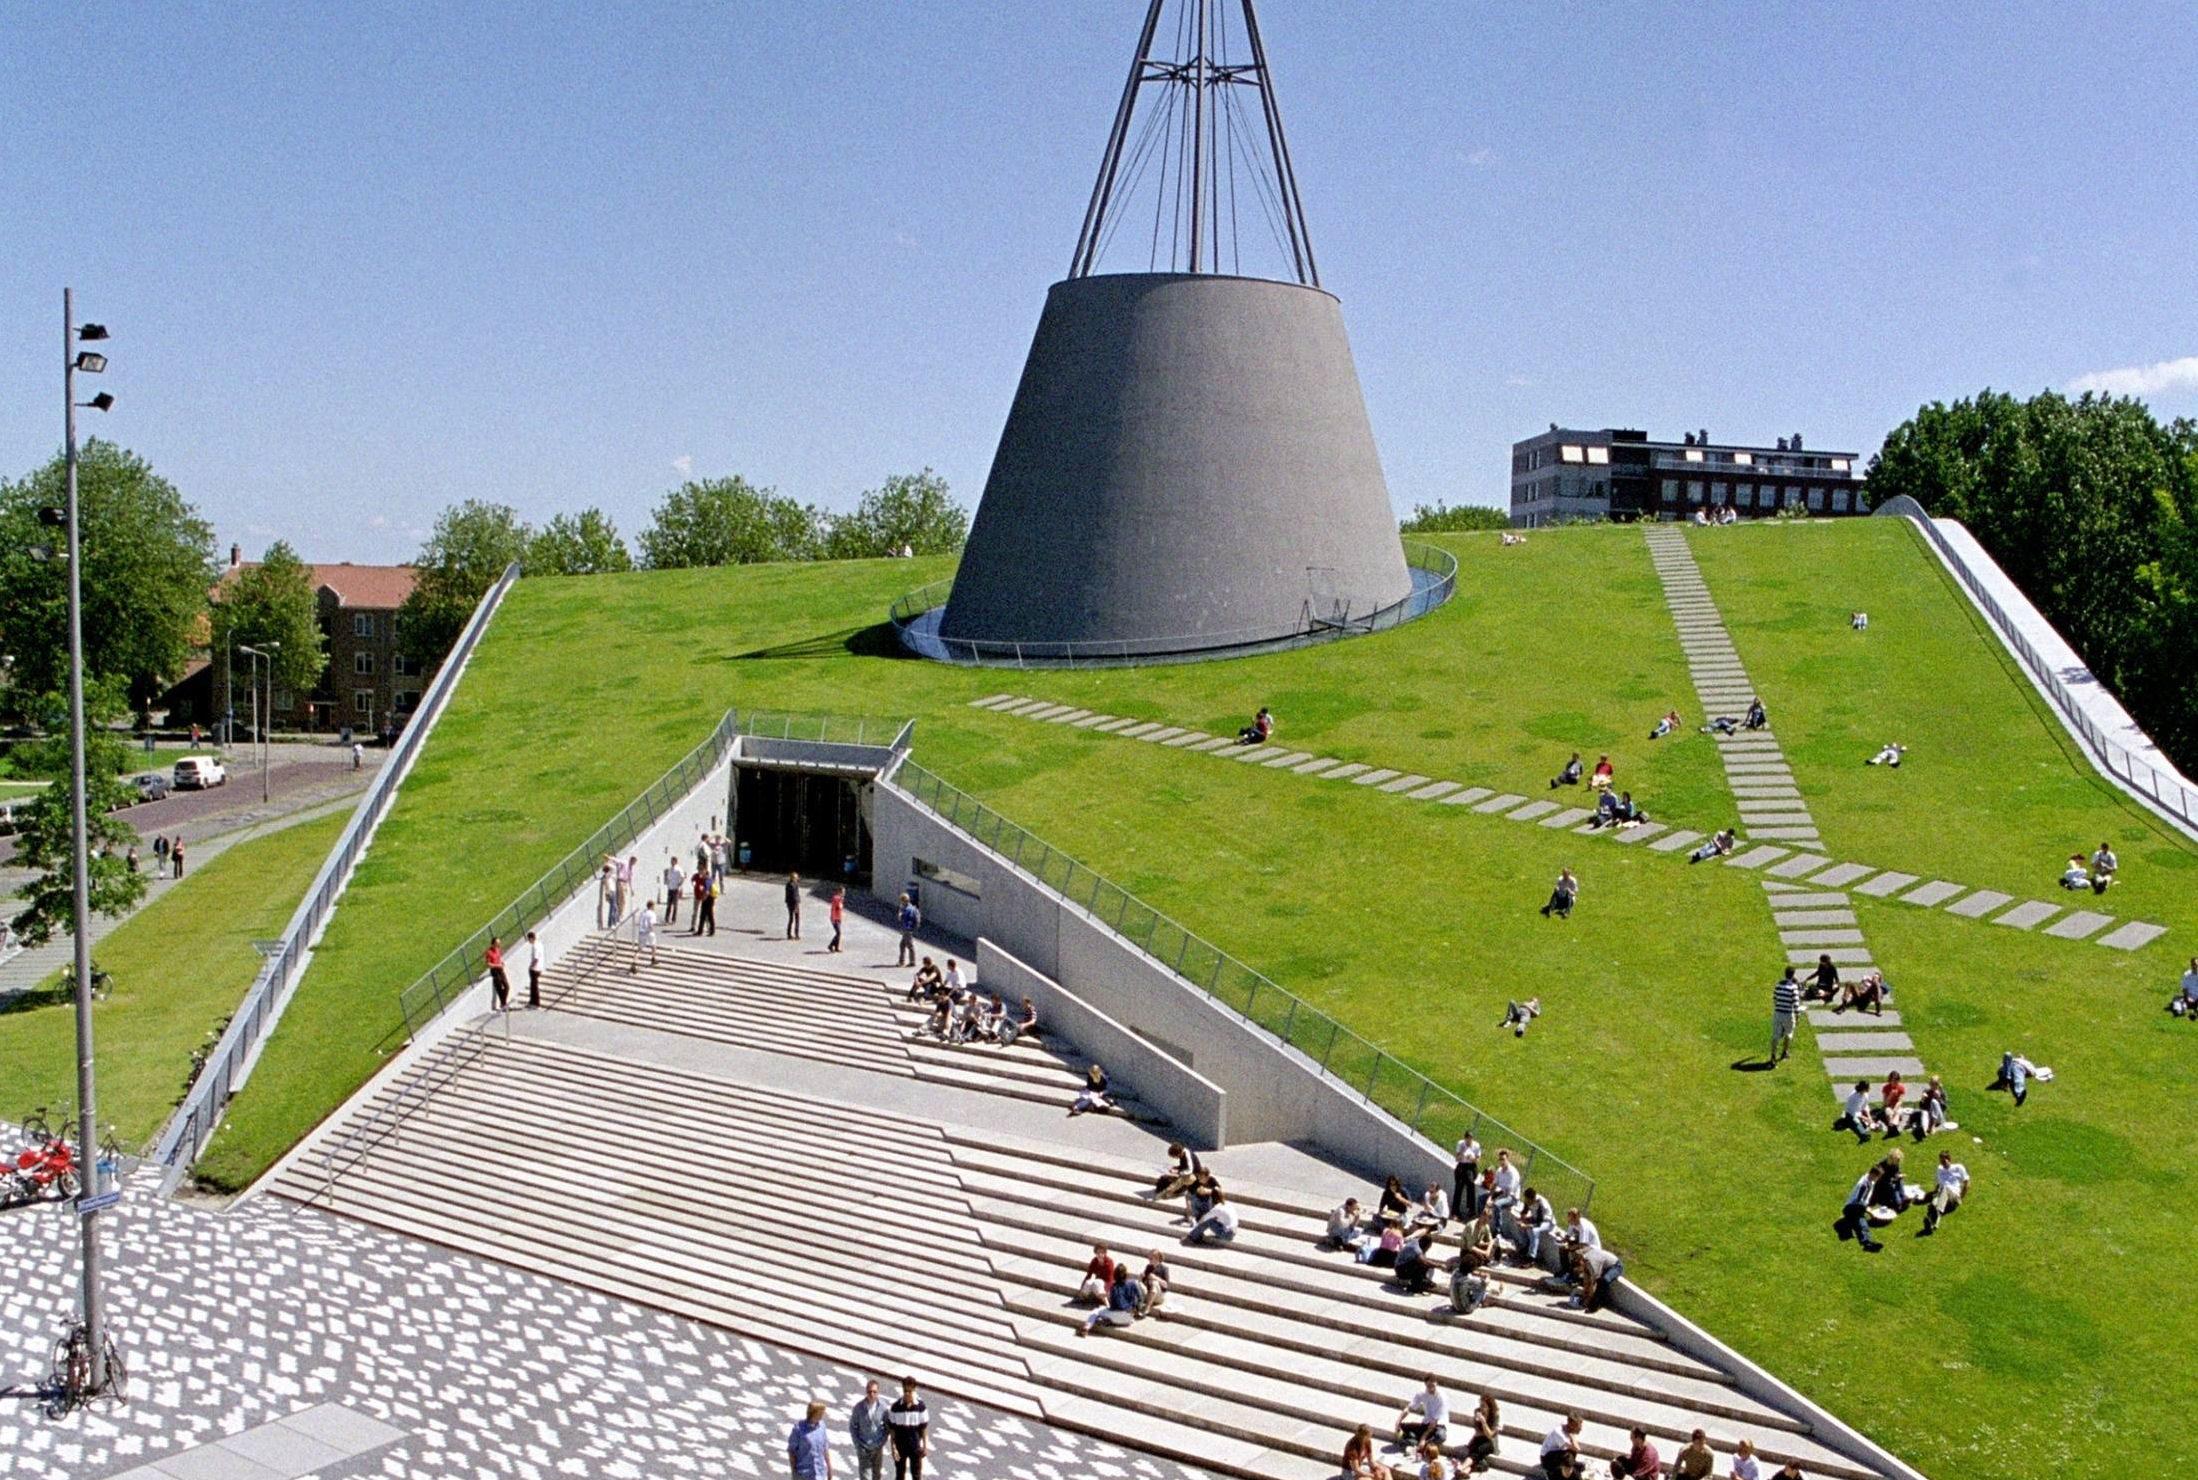
\includegraphics[width=\paperwidth,height=\paperheight]{images/background-titlepage.jpg}}%
\setbeamertemplate{footline}{\usebeamertemplate*{minimal footline}}
\frame{\titlepage}
}

\begin{frame}\frametitle{Inhoud}
    \begin{itemize}
        \item Opdrachtgevers
        \item Opdrachtomschrijving
        \begin{itemize}
        	\item Beschrijving Roosters
        	\item Voorbeeld Demo
        	\item Eisen van de Opdrachtgever
        \end{itemize}
        \item Aanpak en Hulpmiddelen
        \item Flexibiliteit
        \item Linear Programming
        \item Chaining Algoritme
        \item Andere Features
        \item Eind Demo
        \item Vragen
    \end{itemize}
\end{frame}

\section{Inleiding}
Dit verslag is het eindresultaat van het Bachelorproject in opdracht van NedTrain B.V. en de Technische Universiteit Delft. Het project was gericht op het uitbreiden en verbeteren van software voor een applicatie, de NedTrain Planner, die roosterproblemen kan oplossen en de uitkomsten hiervan op een overzichtelijk manier visualiseren. De applicatie kan voor verschillende doeleinden gebruikt worden door zowel NedTrain als de TU Delft. Er moet dus tijdens het project rekening worden gehouden met verschillende belangen en wensen van beide opdrachtgevers.

In de komende hoofdstukken zal de opdracht en het proces eromheen beschreven worden. Allereerst zal er gedefini\"eerd worden wat het probleem van de opdrachtgevers is. Vervolgens zal het hoofdstuk probleemanalyse gericht zijn op het analyseren en oplossen van het gedefini\"eerde probleem van de opdrachtgevers. Daarna zullen in het hoofdstuk ontwerp de ontwerpkeuzes genoemd en toegelicht worden en komen in het daarop volgende hoofdstuk alle opgeleverde producten en diensten aan bod. Omdat de applicatie gericht is op het oplossen van problemen zal er ook een hoofdstuk gewijd zijn aan de performance van de opgeleverde producten. Vervolgens zal besproken worden hoe het ontwikkelproces gelopen is en wat voor hulpmiddelen er gebruikt zijn. Tenslotte zullen er functionaliteiten aanbevolen worden die eventueel later nog ge\"implementeerd kunnen worden en wordt in de conclusie teruggekeken op het project en een conclusie getrokken met betrekking tot de eisen van het project. Als voorbereiding op dit project zijn in de eerste weken een aantal documenten opgesteld, namelijk een Plan van Aanpak \emph{(zie bijlage \ref{app:B})}, een Ori\"entatieverslag \emph{(zie bijlage \ref{app:C})} en een Requirementsanalyse \emph{(zie Bijlage \ref{app:D})}

De volgende paragrafen zullen een korte inleiding geven over het bedrijf NedTrain en waarom de NedTrain Planner relevant is voor hen en de TU Delft.

\subsection{NedTrain}
Het bedrijf NedTrain is een dochterbedrijf van de Nederlandse Spoorwegen (NS), net als bijvoorbeeld NS Reizigers B.V., de verantwoordelijke voor het personenvervoer. NedTrain is het dochterbedrijf dat zorgt voor het onderhoud aan alle treinen aangeleverd door NS Reizigers. Dat onderhoud bestaat niet alleen uit het repareren, maar ook uit het reinigen en moderniseren van treinen. Er moet hierbij gezorgd worden dat van de grofweg 3000 bestaande treinstellen bij NS er op elk moment genoeg beschikbaar zijn om gebruikt te kunnen worden door NS Reizigers. Om dit te bereiken staan er op elk moment van de dag ongeveer 250 treinstellen tegelijk voor onderhoud op meer dan 30 locaties door heel Nederland in de werkplaatsen van NedTrain. Hier werken in totaal ongeveer 3500 mensen 24 uur per dag, 7 dagen per week aan de opgenoemde taken. Het hoofdkantoor van NedTrain staat in Utrecht.

\subsection{NedTrain Planner}
Vanwege de omvang van de activiteiten, die NedTrain dagelijks moet afhandelen, worden er roosters gemaakt die een weergave van de dag geven en er voor moeten zorgen dat deze activiteiten op tijd uitgevoerd worden. Dit is een uitputtende taak en alhoewel NedTrain in het bezit is van software moet er nog steeds veel met de hand worden gedaan. Om NedTrain te helpen bij het inzicht geven van de nieuwste ontwikkelingen rondom het oplossen van moeilijke roosterproblemen is er in samenwerking met de TU Delft de NedTrain Planner ontwikkeld, dat het resultaat is van meerdere projecten van studenten aan de TU Delft. Roostermakers bij NedTrain zouden deze applicatie kunnen gebruiken om hun werkverrichtingen te vergemakkelijken en hun denkwijze te verbeteren. Daarnaast biedt het voor de TU Delft een educatief demonstratiemiddel voor onderzoek, doordat de applicatie visueel goed kan laten zien hoe de oplossing door een algoritme tot stand komt en hoe dus een dergelijk algoritme werkt.

\begin{frame}\frametitle{Opdrachtgevers}
\begin{columns}[T] % align columns
    \begin{column}{.55\textwidth}
        \begin{itemize}
            \item NedTrain 
            \begin{itemize}
                \item Nederlandse Spoorwegen
                \item $250$ treinen op $30$ locaties
                \item $3500$ werknemers
                \item ir. Bob Huisman
            \end{itemize}
        \end{itemize}
        \vspace{1.8cm}
        \begin{itemize}
            \item TU Delft
            \begin{itemize}
                \item Algoritmiek groep
                \item prof. dr. Cees Witteveen
            \end{itemize}  
        \end{itemize}
    \end{column}%
    \begin{column}{.45\textwidth}
        
\includegraphics[width=4.5cm]{images/logo-nedtrain.jpg}
        \vspace{1cm}
        
\includegraphics[width=5cm]{images/tudelft_logo.pdf}
    \end{column}%
\end{columns}
\end{frame}


\begin{frame}\frametitle{Flexibiliteit (1)}
    \begin{itemize}
        \item Hoe wordt flexibiliteit gemeten?
        \begin{itemize}
            \item<4-> Voor \'e\'en taak: $flex_t = t^+ - t^-$
        \end{itemize}
    \end{itemize}

    \newcommand{\widthpic}{100mm}
    \newcommand{\heightpic}{10mm}
    \newcommand{\offset}{2mm}
    \begin{tikzpicture}
        \coordinate (A) at (0, \heightpic /2);
        \coordinate (B) at (\widthpic, \heightpic /2);
        \coordinate (A1) at (0, 0);
        \coordinate (A2) at (0, \heightpic);
        \coordinate (B1) at (\widthpic, 0);
        \coordinate (B2) at (\widthpic, \heightpic);

        \draw [very thick] (A) -- (B);

        \filldraw[very thick, draw=darkgreen,fill=lightgreen, visible on=<1>] (10mm, \offset) rectangle (35mm, 8mm);
        \filldraw[very thick, draw=darkgreen,fill=lightgreen, visible on=<2>] (0mm, \offset) rectangle (25mm, 8mm);
        \filldraw[very thick, draw=darkgreen,fill=lightgreen, visible on=<3->] (75mm, \offset) rectangle (100mm, 8mm);

        \node[visible on=<2->] at (0mm,-3mm) {$t^-$};
        \node[visible on=<3->] at (75mm,-3mm) {$t^+$};

        \draw [very thick] (A1) -- (A2);
        \draw [very thick] (B1) -- (B2);
    \end{tikzpicture}
\end{frame}

\begin{frame}\frametitle{Flexibiliteit (2)}
    \begin{itemize}
        \item Hoe wordt flexibiliteit gemeten?
        \begin{itemize}
            \item Voor \'e\'en taak: $flex_t = t^+ - t^-$
            \item Voor hele schema: $flex_{totaal} = \sum_{t \in T}(t^+ - t^-)$    
            \item<2-> Voorrangsrelatie: $a \prec b$
        \end{itemize}
    \end{itemize}

    \newcommand{\widthpic}{100mm}
    \newcommand{\offset}{2mm}
    \begin{tikzpicture}
        \coordinate (A) at (0, 17mm);
        \coordinate (B) at (\widthpic, 17mm);
        \coordinate (A1) at (0, 12mm);
        \coordinate (A2) at (0, 22mm);
        \coordinate (B1) at (\widthpic, 12mm);
        \coordinate (B2) at (\widthpic, 20mm);

        \coordinate (C) at (0, 5mm);
        \coordinate (D) at (\widthpic, 5mm);
        \coordinate (C1) at (0, 0mm);
        \coordinate (C2) at (0, 10mm);
        \coordinate (D1) at (\widthpic, 0mm);
        \coordinate (D2) at (\widthpic, 10mm);

        \draw [very thick] (A) -- (B);
        \draw [very thick] (C) -- (D);

        \node at (-5mm,17mm) {$a$};
        \node at (-5mm,5mm) {$b$};

        % ergens in het midden
        \filldraw[very thick, draw=darkgreen,fill=lightgreen, visible on=<1-2>] (10mm, 14mm) rectangle (35mm, 20mm);
        \filldraw[very thick, draw=darkyellow,fill=lightyellow, visible on=<1-2>] (55mm, 2mm) rectangle (75mm, 8mm);

        % aan het begin
        \filldraw[very thick, draw=darkgreen,fill=lightgreen, visible on=<3>] (0mm, 14mm) rectangle (25mm, 20mm);
        \filldraw[very thick, draw=darkyellow,fill=lightyellow, visible on=<3>] (25mm, 2mm) rectangle (45mm, 8mm);

        % aan het einde
        \filldraw[very thick, draw=darkgreen,fill=lightgreen, visible on=<4->] (55mm, 14mm) rectangle (80mm, 20mm);
        \filldraw[very thick, draw=darkyellow,fill=lightyellow, visible on=<4->] (80mm, 2mm) rectangle (100mm, 8mm);
        
        % curly bracket
        \draw [decorate,decoration={brace,amplitude=10pt}, visible on=<5>]
        (0mm,23mm) -- (55mm,23mm) node [black,midway, yshift=6mm] 
        {\footnotesize $flex_{totaal}$};

        \draw [very thick] (A1) -- (A2);
        \draw [very thick] (B1) -- (B2);
        \draw [very thick] (C1) -- (C2);
        \draw [very thick] (D1) -- (D2);

        \draw [very thick, ->, visible on=<2>] (22mm, 17mm) -- (65mm, 5mm);
        \draw [very thick, ->, visible on=<3>] (12.5mm, 17mm) -- (35mm, 5mm);
        \draw [very thick, ->, visible on=<4->] (67.5mm, 17mm) -- (90mm, 5mm);
    \end{tikzpicture}
\end{frame}

\begin{frame}\frametitle{Flexibiliteit (3)}
    \begin{itemize}
        \item Voor hele schema: $flex_{totaal} = \sum_{t \in T}(t^+ - t^-)$
        \item Onafhankelijke intervallen
    \end{itemize}

    \newcommand{\widthpic}{100mm}
    \newcommand{\offset}{2mm}
    \begin{tikzpicture}
        \coordinate (A) at (0, 17mm);
        \coordinate (B) at (52.5mm, 17mm);
        \coordinate (A1) at (0, 12mm);
        \coordinate (A2) at (0, 22mm);
        \coordinate (B1) at (52.5mm, 12mm);
        \coordinate (B2) at (52.5mm, 20mm);

        \coordinate (C) at (52.5mm, 5mm);
        \coordinate (D) at (\widthpic, 5mm);
        \coordinate (C1) at (52.5mm, 0mm);
        \coordinate (C2) at (52.5mm, 10mm);
        \coordinate (D1) at (\widthpic, 0mm);
        \coordinate (D2) at (\widthpic, 10mm);

        \draw [very thick] (A) -- (B);
        \draw [very thick] (C) -- (D);

        \node at (-5mm,17mm) {$a$};
        \node at (-5mm,5mm) {$b$};

        % ergens in het midden
        \filldraw[very thick, draw=darkgreen,fill=lightgreen] (10mm, 14mm) rectangle (35mm, 20mm);
        \filldraw[very thick, draw=darkyellow,fill=lightyellow] (55mm, 2mm) rectangle (75mm, 8mm);
        
        \draw [very thick] (A1) -- (A2);
        \draw [very thick] (B1) -- (B2);
        \draw [very thick] (C1) -- (C2);
        \draw [very thick] (D1) -- (D2);
    \end{tikzpicture}
\end{frame}

\begin{frame}\frametitle{Linear Programming}
    \begin{definitie}
        \begin{align}
            \text{max:}& \quad \sum_{t \in T} (t^+ - t^-) & \nonumber \\
            % constraint 1
            \only<1>{\phantom{\text{met voorwaarden:}} & \phantom{\quad t^- \leq t^+} & \phantom{\forall t \in T} \nonumber \\}
            \only<2->{\text{met voorwaarden:} & \quad t^- \leq t^+ & \forall t \in T \nonumber \\} 
            % contraint 2
            \only<-2>{& \phantom{\quad a^+ - b^- \leq -d_a} & \phantom{\forall (a \prec b) \in C} \nonumber}
            \only<3-8>{& \phantom{\quad a^+ - b^- \leq -d_a} & \forall (a \prec b) \in C \nonumber}
            \only<9->{& \quad a^+ + d_a \leq b^- & \forall (a \prec b) \in C \nonumber}
        \end{align}
    \end{definitie}

    \begin{itemize}
        \item \only<4->{$a \prec b$} \only<8->{$\quad \Rightarrow \quad a^+ + d_a \leq b^-$}
        \item<10-> COIN-OR Linear Programming Solver (CLP)
    \end{itemize}

    \begin{tikzpicture}
        \draw[very thick, visible on=<4->] (-0.4mm, 2.5mm) -- (100mm, 2.5mm);
        \draw[very thick, visible on=<4->] (-0.4mm, 0mm) -- (-0.4mm, 5mm);
        \draw[very thick, visible on=<4->] (100mm, 0mm) -- (100mm, 5mm);

        \filldraw[very thick, draw=darkgreen,fill=lightgreen, visible on=<4-5>] (0mm,0mm) rectangle (40mm,5mm) node[pos=.5] {$a$};
        \filldraw[very thick, draw=darkgreen,fill=lightgreen, visible on=<6->] (10mm,0mm) rectangle (50mm,5mm) node[pos=.5] {$a$};
        \filldraw[very thick, draw=darkyellow,fill=lightyellow, visible on=<4->] (50.4mm,0mm) rectangle (70mm,5mm) node[pos=.5] {$b$};

        \draw [decorate, decoration={brace,amplitude=10pt}, visible on=<5>]
        (0mm,6mm) -- (40mm,6mm) node [black,midway, yshift=6mm] 
        {\footnotesize $d_a$};
\draw [decorate, decoration={brace,amplitude=10pt}, visible on=<6->]
        (10mm,6mm) -- (50mm,6mm) node [black,midway, yshift=6mm] 
        {\footnotesize $d_a$};

        \node[visible on=<5->] at (0mm, -2mm) {$a^-$};
        \node[visible on=<7->] at (10mm, -2mm) {$a^+$};
        \node[visible on=<5->] at (50mm, -2mm) {$b^-$};
    \end{tikzpicture}
\end{frame}

\begin{frame}[fragile]\frametitle{Chaining (1)}
    \begin{itemize}      
        \item Resource conflicten oplossen
        %\item<8-> $a \prec b$
    \end{itemize}
    \vspace{5mm}
    \newcommand{\widthpic}{100mm}
    \newcommand{\heightpic}{30mm}
    \newcommand\dashline[1]{\draw[thick, dashed] (0, #1) -- (100mm, #1)}
    \newcommand\normline[1]{\draw[very thick] (0, #1) -- (100mm, #1)}
    \begin{tikzpicture}
        \coordinate (A) at (0, 0);
        \coordinate (B) at (\widthpic, 0);
        \coordinate (C) at (\widthpic, \heightpic);
        \coordinate (D) at (0, \heightpic);

        % onder de resources
        % taak A
        \filldraw[very thick, draw=darkgreen,fill=lightgreen, visible on=<2-3>] (17.5mm, -15mm) rectangle (47.5mm, -5mm) node[pos=.5] {$R_2$};
        \filldraw[very thick, draw=darkgreen,fill=lightgreen, visible on=<2-4>] (17.5mm, -25mm) rectangle (47.5mm, -15mm) node[pos=.5] {$R_2$};
        \node[visible on=<2-4>] at (13mm,-15mm) {$a$};

        % taak B
        \filldraw[very thick, draw=darkyellow,fill=lightyellow, visible on=<3-5>] (57.5mm, -15mm) rectangle (82.5mm, -5mm) node[pos=.5] {$R_1$};
        \filldraw[very thick, draw=darkyellow,fill=lightyellow, visible on=<3-6>] (57.5mm, -25mm) rectangle (82.5mm, -15mm) node[pos=.5] {$R_2$};
        \node[visible on=<3-6>] at (86mm,-15mm) {$b$};
            
        % geplaatst
        % taak A
        \filldraw[very thick, draw=darkgreen,fill=lightgreen, visible on=<4->] (0mm, 10mm) rectangle (30mm, 20mm);
        \filldraw[very thick, draw=darkgreen,fill=lightgreen, visible on=<5->] (0mm, 0mm) rectangle (30mm, 10mm);

        % taak B
        \filldraw[very thick, draw=darkyellow,fill=lightyellow, visible on=<6>] (0mm, 20mm) rectangle (25mm, 30mm);
        \filldraw[very thick, draw=darkyellow,fill=lightyellow, visible on=<7->] (40mm, 20mm) rectangle (65mm, 30mm);
        \filldraw[very thick, draw=darkyellow,fill=lightyellow, visible on=<7->] (40mm, 10mm) rectangle (65mm, 20mm);

        \draw[very thick] (A) rectangle (C);

        \dashline{1 * \heightpic / 3};
        \normline{2 * \heightpic / 3};

        \node at (-5mm, 25mm) {$R_1$};
        \node at (-5mm, 10mm) {$R_2$};
        
        \draw [->, very thick, visible on=<8->] (25mm, 15mm) -- (45mm, 15mm);
    \end{tikzpicture}
\end{frame}

\begin{frame}[fragile]\frametitle{Chaining (1)}
	\addtocounter{framenumber}{-1}
    \begin{itemize}      
        \item Resource conflicten oplossen
    \end{itemize}
    \vspace{5mm}
    \newcommand{\widthpic}{100mm}
    \newcommand{\heightpic}{30mm}
    \newcommand\dashline[1]{\draw[thick, dashed] (0, #1) -- (100mm, #1)}
    \newcommand\normline[1]{\draw[very thick] (0, #1) -- (100mm, #1)}
    \begin{tikzpicture}
        \coordinate (A) at (0, 0);
        \coordinate (B) at (\widthpic, 0);
        \coordinate (C) at (\widthpic, \heightpic);
        \coordinate (D) at (0, \heightpic);
            
        % geplaatst
        % taak A
        \filldraw[very thick, draw=darkgreen,fill=lightgreen] (0mm, 10mm) rectangle (30mm, 20mm);
        \filldraw[very thick, draw=darkgreen,fill=lightgreen] (0mm, 0mm) rectangle (30mm, 10mm);

        % taak B
        \filldraw[very thick, draw=darkyellow,fill=lightyellow] (40mm, 20mm) rectangle (65mm, 30mm);
        \filldraw[very thick, draw=darkyellow,fill=lightyellow] (40mm, 10mm) rectangle (65mm, 20mm);

        \draw[very thick] (A) rectangle (C);

        \dashline{1 * \heightpic / 3};
        \normline{2 * \heightpic / 3};

        \node at (-5mm, 25mm) {$R_1$};
        \node at (-5mm, 10mm) {$R_2$};
        
        \draw [->, very thick] (25mm, 15mm) -- (45mm, 15mm);
    \end{tikzpicture}
    
    \begin{itemize}
    		\item $a \prec b$
    \end{itemize}
    
    \vspace{16mm}
\end{frame}
	
\begin{frame}[fragile] \frametitle{Chaining (2)}
    \newcommand{\widthpic}{100mm}
    \newcommand{\heightpic}{30mm}
    \newcommand\dashline[1]{\draw[thick, dashed] (0, #1) -- (100mm, #1)}
    \newcommand\normline[1]{\draw[very thick] (0, #1) -- (100mm, #1)}
    
	\begin{itemize}
		\item Minimaliseren van het aantal constraints.
	\end{itemize}
	\vspace{5mm}
    
	\begin{tikzpicture}
        \coordinate (A) at (0, 0);
        \coordinate (B) at (\widthpic, 0);
        \coordinate (C) at (\widthpic, \heightpic);
        \coordinate (D) at (0, \heightpic);
            
        % geplaatst
        % taak A
        \filldraw[very thick, draw=darkgreen,fill=lightgreen] (0mm, 10mm) rectangle (30mm, 20mm);
        \filldraw[very thick, draw=darkgreen,fill=lightgreen] (0mm, 0mm) rectangle (30mm, 10mm);

        % taak B
        \filldraw[very thick, draw=darkyellow,fill=lightyellow] (40mm, 20mm) rectangle (65mm, 30mm);
        \filldraw[very thick, draw=darkyellow,fill=lightyellow] (40mm, 10mm) rectangle (65mm, 20mm);
        
        % niet geplaatst
        % taak C
        \filldraw[very thick, draw=darkcyan,fill=lightcyan, visible on=<1>] (70mm, -15mm) rectangle (90mm, -5mm) node[pos=.5] {$R_1$};
        \filldraw[very thick, draw=darkcyan,fill=lightcyan, visible on=<1-3>] (70mm, -25mm) rectangle (90mm, -15mm) node[pos=.5] {$R_2$};
        \node[visible on=<1-3>] at (65mm,-15mm) {$c$};
        
        % wel geplaatst
        % taak C
        \filldraw[very thick, draw=darkcyan,fill=lightcyan, visible on=<2->] (75mm, 20mm) rectangle (95mm, 30mm);
        \filldraw[very thick, draw=darkcyan,fill=lightcyan, visible on=<4->] (75mm, 10mm) rectangle (95mm, 20mm);

        \draw[very thick] (A) rectangle (C);

        \dashline{1 * \heightpic / 3};
        \normline{2 * \heightpic / 3};

        \node at (-5mm, 25mm) {$R_1$};
        \node at (-5mm, 10mm) {$R_2$};
        
        \draw [->, very thick, visible on=<3->] (60mm, 25mm) -- (80mm, 25mm);
        \draw [->, very thick, visible on=<5->] (60mm, 15mm) -- (80mm, 15mm);
        \draw [->, very thick] (25mm, 15mm) -- (45mm, 15mm);
        %\draw [->, very thick, visible on=<2>] (60mm, 15mm) -- (70mm, -15mm);
    \end{tikzpicture}
\end{frame}

\begin{frame}\frametitle{Intercace}
\begin{itemize}
    \item Taken/treinen rooster
    \item Resource profiles
    \item Resource unit rooster
    \item Flexibiliteitsintervallen
\end{itemize}
\end{frame}

\begin{frame}\frametitle{Demo}
    \huge{\hfill Tijd voor een demo! \hfill}
\end{frame}

\begin{frame}\frametitle{Vragen}
    {\hfill%
    
\begin{tikzpicture}[thick,scale=5, every node/.style={transform shape}]
        \node at (0,0.7) {\Huge{Q}};
        \node at (0.45,0.9) {\huge{\&}};
        \node at (0.32,0.35) {\Huge{A}};
    \end{tikzpicture}%
    \hfill%
    }
\end{frame}


\end{document}
